\documentclass{beamer}

% Required packages
\usepackage{fontspec}
\usepackage{fontawesome}
\usepackage{parskip}
\usepackage{hyperref}
\hypersetup{
  colorlinks=false,
  linkbordercolor={white}
}
\usepackage{bookmark}
\usepackage{url}
\usetheme{metropolis}           

\title{AMSE - \textit{MeinBundestag}}
\date{February 3, 2020}
\author{Benjamin Fischer}
\institute{\faInstitution{}\quad{}Friedrich-Alexander Universität Erlangen-Nürnberg}
\newcounter{index}
\stepcounter{index}


\begin{document}
  \maketitle

  \begin{frame}[plain]{MeinBundestag}
    \begin{itemize}
      \item[\faEnvelope]\quad
      \texttt{benjamin.f.fischer@fau.de}
      \item[\faGithub]\quad
      \href{https://github.com/fischerbenjamin/meinbundestag}{\texttt{fischerbenjamin/meinbundestag}}
      \item[\faCopyright]\quad
      \texttt{MIT License}
      \item[\faCogs]\quad
      \texttt{development, not standalone}
    \end{itemize} 
  \end{frame}

  \section{Motivation}
  \begin{frame}[plain]{Motivation}
    \begin{itemize}
      \item[\faInfoCircle]\quad
      \textbf{Idea}
      \begin{itemize}
        \item Informative application about the German parliament
        \item Running on a mobile device (Android/iOS)
      \end{itemize}
      \item[\faBars]\quad
      \textbf{Features}
      \begin{itemize}
        \item Search for a certain deputy or location
        \item Receive general information about the deputy
        \item Read the speeches held by the deputy in the parliament
      \end{itemize}
      \item[\faHeart]\quad
      \textbf{Goal}
      \begin{itemize}
        \item Provide information the user otherwise would not look for
        \item Increase political interest
      \end{itemize}
    \end{itemize}
  \end{frame}

  \section{Demo}

  \section{OpenData}
  \begin{frame}[plain]{OpenData}
    \textbf{\faAt}\quad\textbf{www.bundestag.de/services/opendata}
    \begin{itemize}
      \item Protocols of the parliament given as \texttt{.xml} files
      \item Providing an additional \texttt{.dtd} file for processing
      \item Current election period (since 2017)
      \item Files are updated according to the session schedule
    \end{itemize}
    \textbf{\faExclamationTriangle}\quad\textbf{Problems}
    \begin{itemize}
      \item Only the latest five protocols are included in the table
      \item Loading other protocols requires user interaction
    \end{itemize}  
  \end{frame}

  \begin{frame}[plain]{OpenData}
    \textbf{\faAt}\quad\textbf{www.abgeordnetenwatch.de/api/parliament/bundestag}
    \begin{itemize}
      \item Information about each deputy of the parliament
      \item Votings, secondary activities, etc.
      \item List of all deputies: \path{/deputies.json} 
      \item A deputy's profile: \path{profile/<deputy>/profile.json}
    \end{itemize}
  \end{frame}

  \section{Technology}
  \begin{frame}[plain]{Technology}
    \begin{center}
      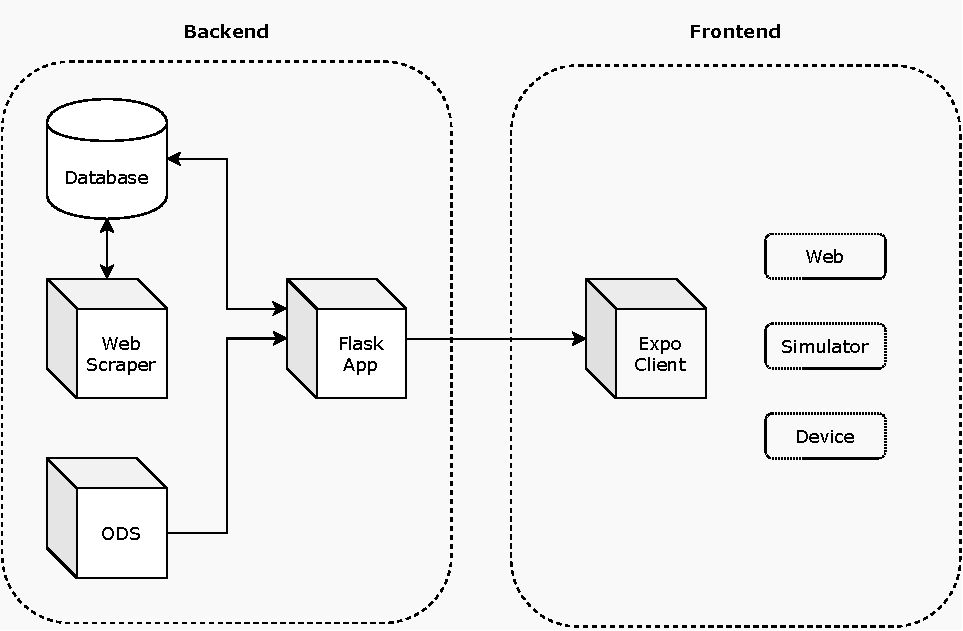
\includegraphics[width=0.99\textwidth]{fig/technology_overview.pdf}
    \end{center}
  \end{frame}

  \begin{frame}[plain]{Technology}
    \textbf{\faDesktop}\quad\textbf{Frontend}
    \begin{itemize}
      \item React Native\textsuperscript{\hyperlink{link-react-native}{\arabic{index}}} application
      \stepcounter{index}
      \item Usage of Expo\textsuperscript{\hyperlink{link-expo}{\arabic{index}}} for easier development
      \stepcounter{index}
      \item Minimalistic, platform-independent code
    \end{itemize}
    \textbf{\faServer}\quad\textbf{Backend}
    \begin{itemize}
      \item Python Flask\textsuperscript{\hyperlink{link-flask}{\arabic{index}}} application provides the API
      \stepcounter{index}
      \item Selenium\textsuperscript{\hyperlink{link-selenium}{\arabic{index}}} web scraper searching for new protocols
      \stepcounter{index}
      \item MongoDB\textsuperscript{\hyperlink{link-mongodb}{\arabic{index}}} database persists processed protocol data
      \stepcounter{index}
      \item Database and API are running in seperate Docker\textsuperscript{\hyperlink{link-docker}{\arabic{index}}} containers
    \end{itemize}
  \end{frame}

  \begin{frame}[plain]{Future Work}
    \begin{itemize}
      \item[\footnotesize{\faWarning}]\enspace{}Run the backend on a public server
      \item[\footnotesize{\faWarning}]\enspace{}Check responsive layout, fix some layout bugs
      \item[\footnotesize{\faStar}]\enspace{}Support more parliaments
      \item[\footnotesize{\faStar}]\enspace{}Improve the speech analysis
      \item[\footnotesize{\faStar}]\enspace{}Add text-to-speech functionality for speeches
      \item[\footnotesize{\faStar}]\enspace{}Expand search by parties, topic, period of time 
      \item[\footnotesize{\faStar}]\enspace{}Include some animations for better user experience
    \end{itemize}
  \end{frame}

  \section{ODS}
  \begin{frame}[plain]{ODS}
    \,\textbf{\faUser}\quad\textbf{Specific}
    \begin{itemize}
      \item The ODS is used for providing the list of all deputies
      \item Not applicable for protocol data (obviously)
      \item Providing profile data would require supporting placeholders
      \item Easy to setup, my experience from Linux system
    \end{itemize}
    \textbf{\faUsers}\quad\textbf{General}
    \begin{itemize}
      \item Innovative idea, especially for multiple small projects
      \item Beneficial for applications with timeline views / historical data 
    \end{itemize} 
  \end{frame}

  \begin{frame}[plain]{ODS}
    \textbf{\faThumbsUp}\quad\textbf{Suggestions}
    \begin{itemize}
      \item Custom names for storage links of pipelines
      \item Adaptable amount of time how long data is persisted
      \item Supporting query parameters and placeholders in API url 
    \end{itemize} 
  \end{frame}


  \begin{frame}[plain]{}
    \centering
    \Large \textbf{Thank you for your attention!}\\
    \vspace{2em}
    \Large \textbf{Questions?}
  \end{frame}


  \begin{frame}[plain]{Links}
    \begin{itemize}
      \item[\textsuperscript{1}] \label{link-react-native}\href{https://facebook.github.io/react-native}{\texttt{https://facebook.github.io/react-native}}
      \item[\textsuperscript{2}] \label{link-expo}\href{https://expo.io/}{\texttt{https://expo.io/}}
      \item[\textsuperscript{3}] \label{link-flask}\href{https://www.fullstackpython.com/flask.html}{\texttt{https://www.fullstackpython.com/flask.html}}
      \item[\textsuperscript{4}] \label{link-selenium}\href{https://selenium-python.readthedocs.io/}{\texttt{https://selenium-python.readthedocs.io/}}
      \item[\textsuperscript{5}] \label{link-mongodb}\href{https://www.mongodb.com/}{\texttt{https://www.mongodb.com/}}
      \item[\textsuperscript{6}] \label{link-mongodb}\href{https://www.docker.com/}{\texttt{https://www.docker.com/}}
    \end{itemize}
  \end{frame}


\end{document}